In this chapter, we explore three different scenarios that can be achieved by the visualization application. The first demonstrates the influences of the mining strategy, and the second scenario also adds the influences of network delay to the visualization. In addition, the presentation of orphaned blocks and forks proves that the visualization application handles the mining processes correctly. In the last scenario, we explore the limitation of the visualization application.

\section{A Fast Miner}

In the first scenario, there is a fast miner who mines blocks much quicker than the other miners due to the mining strategy. With the low network delay, the fast miner can publish the blocks quickly. Therefore, none of the other miners can compete with the fast miner, i.e., only the fast miner can add blocks to the blockchain.

In this experiment, there are three miners, Alice (red color), Bob (blue color), and Charlie (green color), who compete with each other in the blockchain system. The configuration of this experiment is provided in Configuration File \ref{lst:scenario 1}.

\begin{lstlisting}[caption={Scenario 1}, label={lst:scenario 1}]
{
    "nodes": [
        // transaction generator
        {
            "id": "6f71279b",
            "type": "generator"
        },
        // miner (Alice)
        {
            "id": "f1e50b4f",
            "type": "miner",
            "color": "#e53935",
            "name": "Alice",
            "miningTime": 1,
            "minValue": 1,
            "mineNumber": 1,
            "maxPending": 10
        },
        // miner (Bob)
        {
            "id": "2d30b6fd",
            "type": "miner",
            "color": "#03a9f4",
            "name": "Bob",
            "miningTime": 5,
            "minValue": 4,
            "mineNumber": 3,
            "maxPending": 10
        },
        // miner (Charlie)
        {
            "id": "a6b877ab",
            "type": "miner",
            "color": "#4caf50",
            "name": "Charlie",
            "miningTime": 6,
            "minValue": 7,
            "mineNumber": 2,
            "maxPending": 10
        }
    ],
    "delays": [
        // transaction generator
        {
            "id": "6f71279b",
            "neighbors": [
                {
                    "id": "f1e50b4f",
                    "seconds": 1
                },
                {
                    "id": "2d30b6fd",
                    "seconds": 1
                },
                {
                    "id": "a6b877ab",
                    "seconds": 1
                }
            ]
        },
        // miner (Alice)
        {
            "id": "f1e50b4f",
            "neighbors": [
                {
                    "id": "2d30b6fd",
                    "seconds": 1
                },
                {
                    "id": "a6b877ab",
                    "seconds": 1
                }
            ]
        },
        // miner (Bob)
        {
            "id": "2d30b6fd",
            "neighbors": [
                {
                    "id": "f1e50b4f",
                    "seconds": 1
                },
                {
                    "id": "a6b877ab",
                    "seconds": 1
                }
            ]
        },
        // miner (Charlie)
        {
            "id": "a6b877ab",
            "neighbors": [
                {
                    "id": "f1e50b4f",
                    "seconds": 1
                },
                {
                    "id": "2d30b6fd",
                    "seconds": 1
                }
            ]
        }
    ],
    "transactions": [
        {
            "reward": 2,
            "delay": 0
        },
        {
            "reward": 3,
            "delay": 1
        },
        {
            "reward": 9,
            "delay": 2
        },
        {
            "reward": 4,
            "delay": 3
        },
        {
            "reward": 7,
            "delay": 4
        },
        {
            "reward": 5,
            "delay": 5
        },
        {
            "reward": 1,
            "delay": 6
        },
        {
            "reward": 5,
            "delay": 7
        },
        {
            "reward": 3,
            "delay": 8
        },
        {
            "reward": 2,
            "delay": 9
        }
    ]
}
\end{lstlisting}

As the configuration file shows, Alice's mining strategy is the fastest because the parameters of \textit{Mining Time}, \textit{Minimum Value of Transactions}, and \textit{Fixed Number of Transactions in Blocks} are all set to 1. On the contrary, Bob's and Charlie's parameters are both higher than Alice's parameters. The parameters of network delay are all set to 1. Hence, the blockchain network is stable and fast and it only takes 1 second to publish the blocks to neighbors. For transactions, we defined a sequence of transactions which interval is 1 second.

\begin{figure}[htb]
    \centering
    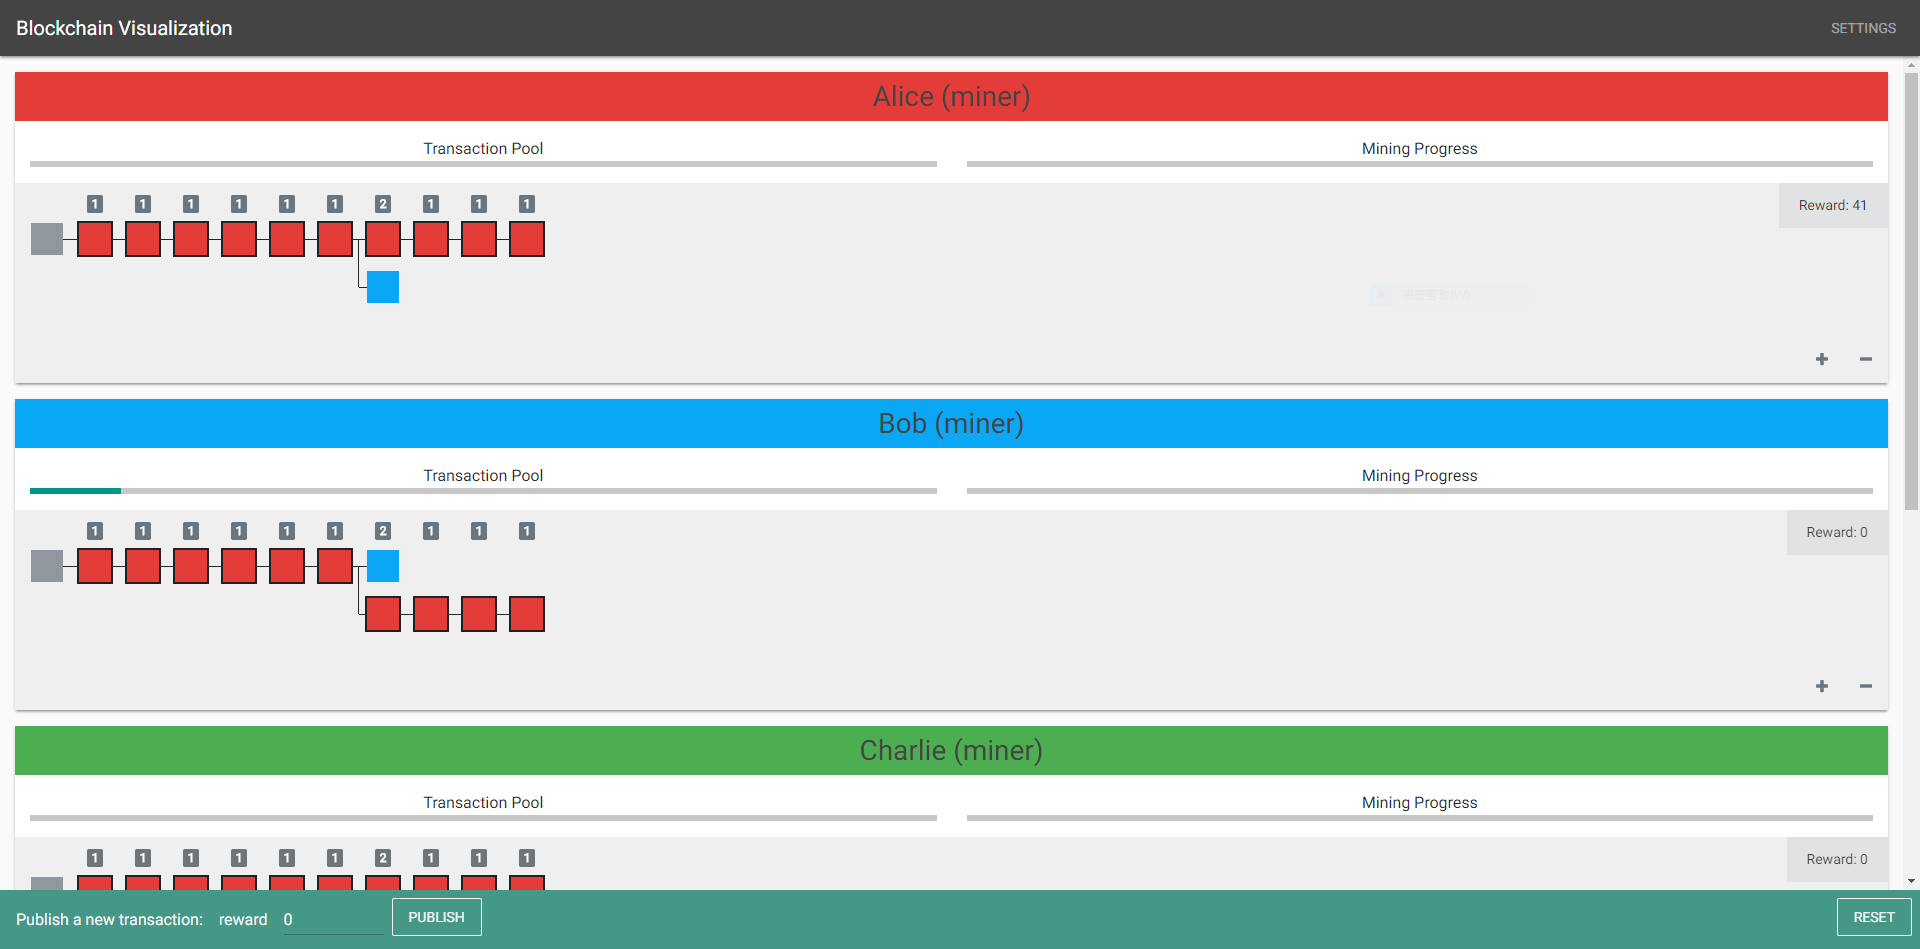
\includegraphics[width=\textwidth]{scenario_case1}
    \caption{Alice was a fast miner.}
    \label{fig:alice was a fast miner}
\end{figure}

In Figure \ref{fig:alice was a fast miner}, it demonstrates the results of the above configuration. Although some transactions have high number of reward, Alice still dominated the blockchain system because of her fast mining strategy. As a result, all of the 10 transactions were mined by Alice, even if Bob tried to mined a block at the seventh layer. 

In summary, this scenario shows the competition between the miners. As our expectation, the mining strategy with the lowest \textit{Mining Time}, \textit{Minimum Value of Transactions} and \textit{Fixed Number of Transactions in Blocks} is the fastest one. Additionally, it shows that the orphaned block were handled by the visualization application correctly, as the fast miner still worked on the correct blockchain data structure.

\section{Multiple Forks}

In the second scenario, there are three miners who have the similar computing power and mining strategies, and compete with each other for a long time. Because the spread of blocks suffers high delays, miners add their own blocks to the blockchain much more quickly than others do. Thus, each miner considers his/her own blockchain is the longest one, and the competition continues. Configuration File \ref{lst:scenario 2} is the configuration file for this scenario.

\begin{lstlisting}[caption={Scenario 2}, label={lst:scenario 2}]
{
    "nodes": [
        // transaction generator
        {
            "id": "6f71279b",
            "type": "generator"
        },
        // miner (Alice)
        {
            "id": "f1e50b4f",
            "type": "miner",
            "color": "#e53935",
            "name": "Alice",
            "miningTime": 1,
            "minValue": 1,
            "mineNumber": 1,
            "maxPending": 10
        },
        // miner (Bob)
        {
            "id": "2d30b6fd",
            "type": "miner",
            "color": "#03a9f4",
            "name": "Bob",
            "miningTime": 1,
            "minValue": 1,
            "mineNumber": 1,
            "maxPending": 10
        },
        // miner (Charlie)
        {
            "id": "a6b877ab",
            "type": "miner",
            "color": "#4caf50",
            "name": "Charlie",
            "miningTime": 1,
            "minValue": 1,
            "mineNumber": 1,
            "maxPending": 10
        }
    ],
    "delays": [
        // transaction generator
        {
            "id": "6f71279b",
            "neighbors": [{
                    "id": "f1e50b4f",
                    "seconds": 1
                },
                {
                    "id": "2d30b6fd",
                    "seconds": 1
                },
                {
                    "id": "a6b877ab",
                    "seconds": 1
                }
            ]
        },
        // miner (Alice)
        {
            "id": "f1e50b4f",
            "neighbors": [{
                    "id": "2d30b6fd",
                    "seconds": 3
                },
                {
                    "id": "a6b877ab",
                    "seconds": 3
                }
            ]
        },
        // miner (Bob)
        {
            "id": "2d30b6fd",
            "neighbors": [{
                    "id": "f1e50b4f",
                    "seconds": 3
                },
                {
                    "id": "a6b877ab",
                    "seconds": 3
                }
            ]
        },
        // miner (Charlie)
        {
            "id": "a6b877ab",
            "neighbors": [{
                    "id": "f1e50b4f",
                    "seconds": 3
                },
                {
                    "id": "2d30b6fd",
                    "seconds": 3
                }
            ]
        }
    ],
    "transactions": [
        {
            "reward": 2,
            "delay": 0
        },
        {
            "reward": 3,
            "delay": 1
        },
        {
            "reward": 9,
            "delay": 2
        },
        {
            "reward": 4,
            "delay": 3
        },
        {
            "reward": 7,
            "delay": 4
        },
        {
            "reward": 5,
            "delay": 5
        },
        {
            "reward": 1,
            "delay": 6
        },
        {
            "reward": 5,
            "delay": 7
        },
        {
            "reward": 3,
            "delay": 8
        },
        {
            "reward": 2,
            "delay": 9
        }
    ]
}
\end{lstlisting}

In the configuration file, Alice's, Bob's and Charlie's parameters of the mining strategy are set to the same value. Therefore, it is expected that the three miners will always mine at the same time. The parameters of the network delay are higher than the parameters of \textit{Mining Time} to simulate the bad network conditions between three miners. The sequence of transactions are the same as Configuration File \ref{lst:scenario 1}.

\begin{figure}[htb]
    \centering
    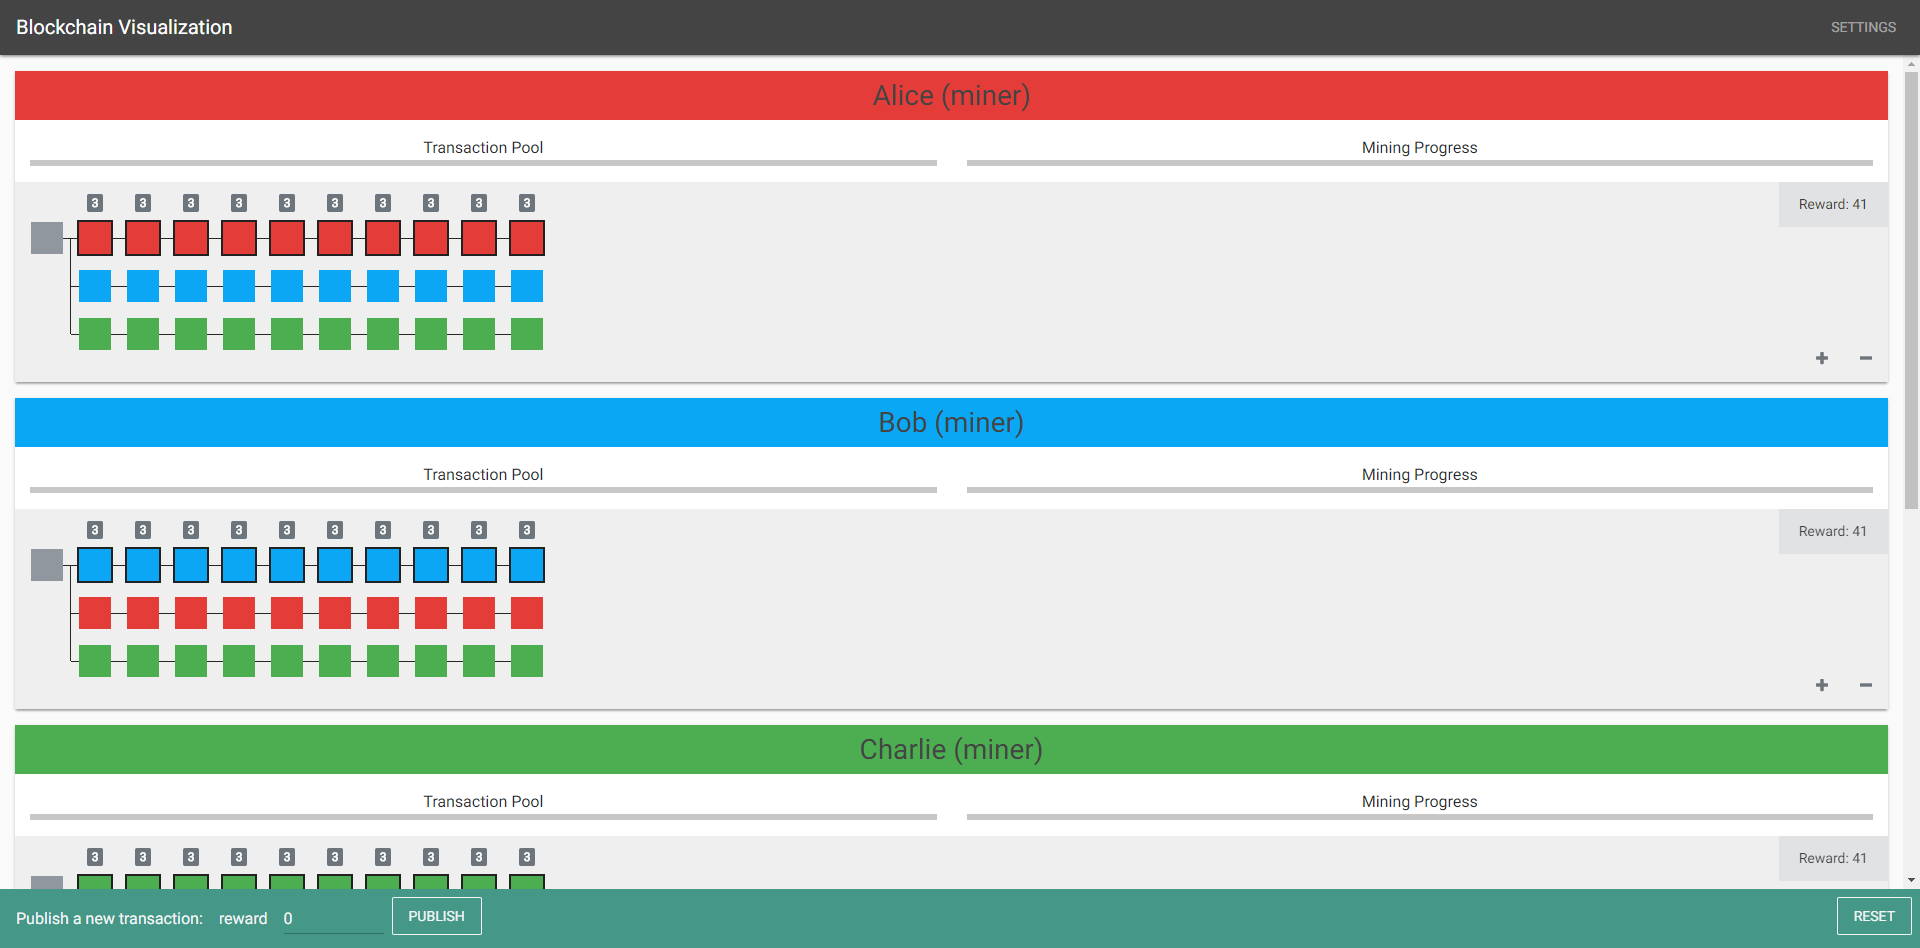
\includegraphics[width=\textwidth]{scenario_case2}
    \caption{Alice, Bob, and Charlie competed with each other.}
    \label{fig:alice, bob, and charlie competed with each other}
\end{figure}

In Figure \ref{fig:alice, bob, and charlie competed with each other}, Alice, Bob, and Charlie compete with each other for a long time because the duration of mining time is shorter than the duration of publishing blocks. The miners are divided into three groups which work on different blockchain data structures because every miner considered that their own blockchain is the lognest. It can be checked that the mining processes visualized the mining processes according to the above description, as Figure \ref{fig:the mining processes of scenario 2} shows.

\begin{figure}[htb]
    \centering
    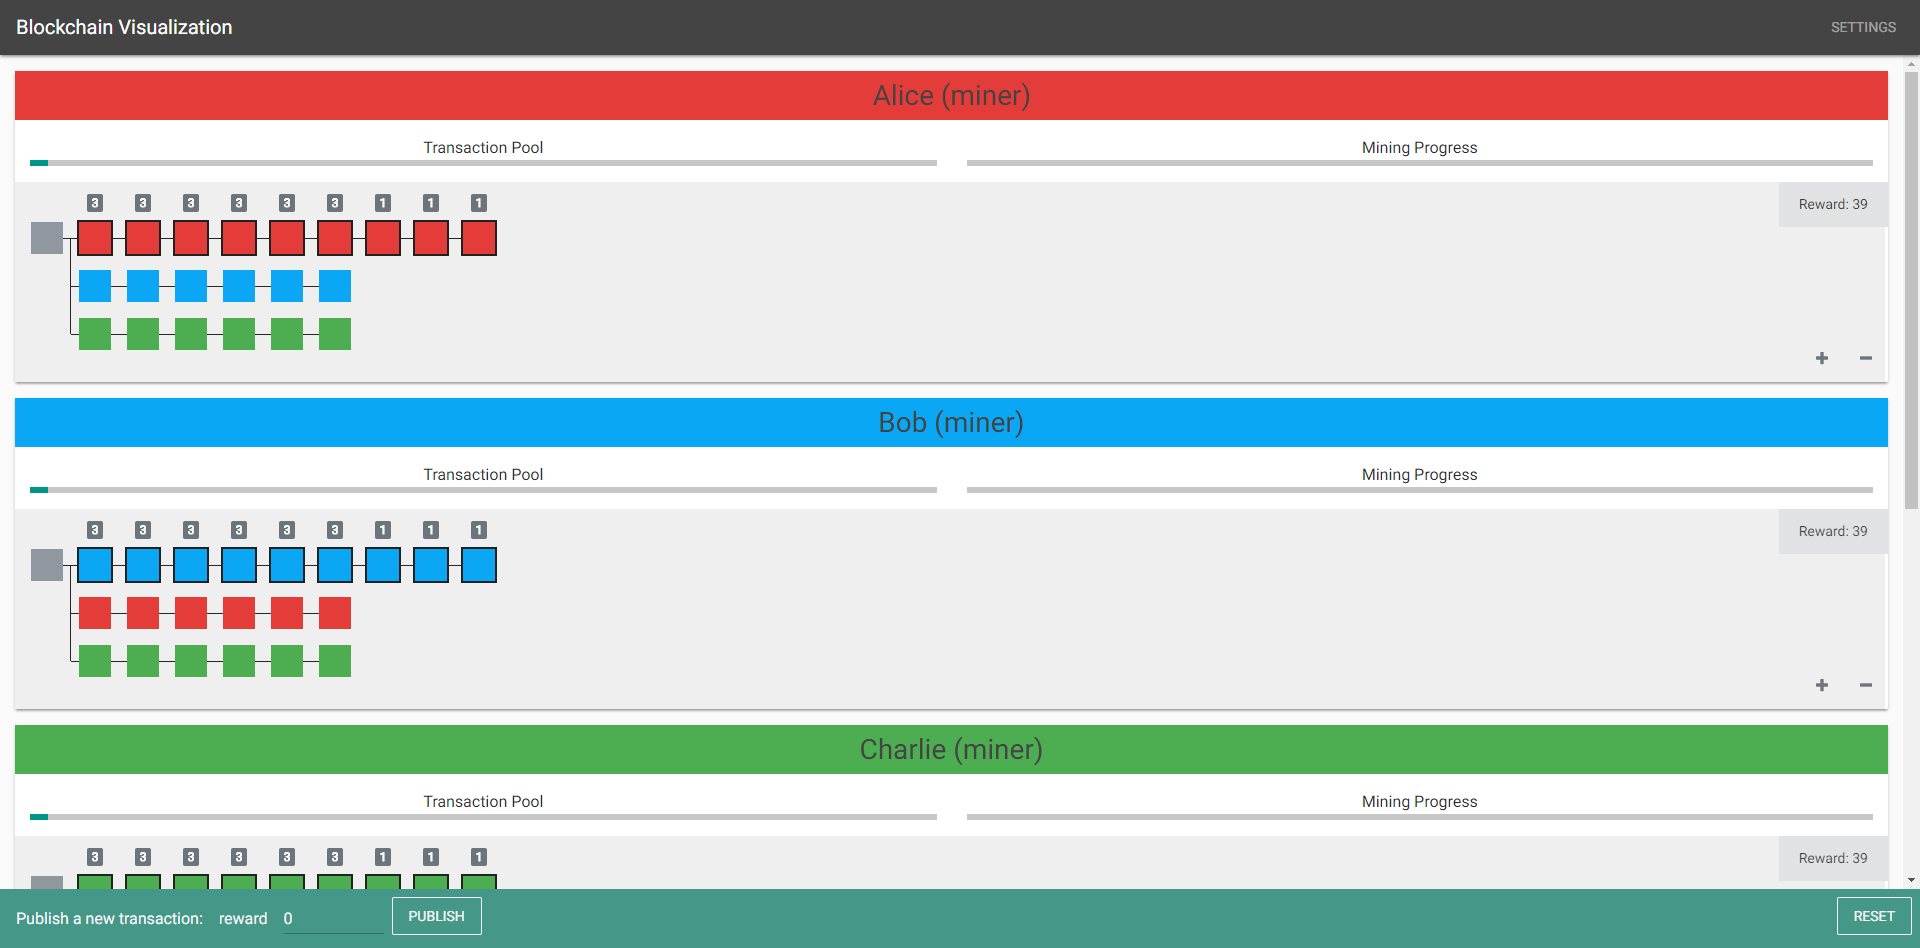
\includegraphics[width=\textwidth]{scenario_case2_2}
    \caption{The mining processes of scenario 2.}
    \label{fig:the mining processes of scenario 2}
\end{figure}

In conclusion, it demonstrates that the visualization application is able to handle the forks correctly. Furthermore, the mining processes are also correct. However, there is a weak point in the visualization application. The forks cannot be merged in the current implementation because the parameters of the mining strategy are fixed during the visualization. Thus, the scenario of multiple forks in the visualization represent the scenario of the hard forks in the real blockchain networks. It should be improved to handle the scenario of the soft forks in the future.

\section{Limitation of Nodes and Transactions}

Through experiments, we found that the maximum number of nodes that can be handled by the application is 15 because of the limitation of the visualization engine, i.e., the Three.js library. The visualization engine cannot created too much canvases due to the performance issue. Hence, the sum of the number of miners and nonminers is limited to 15. On the other hand, the number of transactions that can be handled should be unlimited. We tested it by publishing 100 transactions, and the application still operates correctly.

